\documentclass{article}

\usepackage{graphicx}
\usepackage{gensymb}

\title{Balsa Glider and Flight Dynamics Activity}
\author{Yohannes Kasseya, Micaiah Smith-Pierce, Eric Shen}
\date{\it{12-April-2017}}

\begin{document}
\maketitle

\section{Nomenclature}
\begin{tabular}{l l}
b & span \\
c & chord \\
AR & aspect ratio \\
e & spanwise efficiency factor\\
S & planform area \\
$\alpha$ or AOA & Angle of Attack \\
$C_L$ & Lift Coefficient \\
${C_D}_i$ & Induced Drag Coefficient \\
${C_D}_0$ & Profile Drag Coefficient \\
L & lift force on aircraft\\
D & drag force on aircraft\\
W & gross weight of aircraft\\
CG & Center of gravity\\
m & glide slope.  If the glider travels x meters forward for every y meters down, then $m = -y/x$\\
Re & Reynolds number\\
$\rho$ & air density\\
V & freestream velocity\\
\end{tabular}

\section{Introduction}
 This assignment focused on making a balsa wood glider that is capable of traveling a certain amount of distance in the horizontal direction. In order to maximize the range the glider is able to travel, aerodynamic components and overall design had to be efficient enough to optimize the lift to drag ratio while being stable at the same time. The size and placement of the wings, the angle of attack

and launch, initial velocity (more specifically the power of the throw), and curvature of the wing- that is to minimize induce drag- had to be considered for optimization of the overall design. 

\section{General Overview of the Design}
The designers were provided with a sheet of balsa with a thickness of 1/32" and a length of 16" which was used for wing component of the glider. The designers were also provided with an additional piece of balsa wood with the dimensions of 16"-1/2"-1/4" (length-width-height) which was utilized for the making of the fuselage. The wind of the glider has a chord length value of 2 inches, more specifically a mean value of 1.57 due to its elliptical composition, while having a span of 16”. Given these values, the wing had an area of $25.13 in^3$ and an aspect ratio of 10.19. The fully assembled glider spans 16 inches in length, a maximum width of roughly 16 inches (measured from tip to tip of the wing), and a height of ½ inch at the center of the glider and 2 inches at either end of the wing (this is due to the curvature of the tips of the wing).

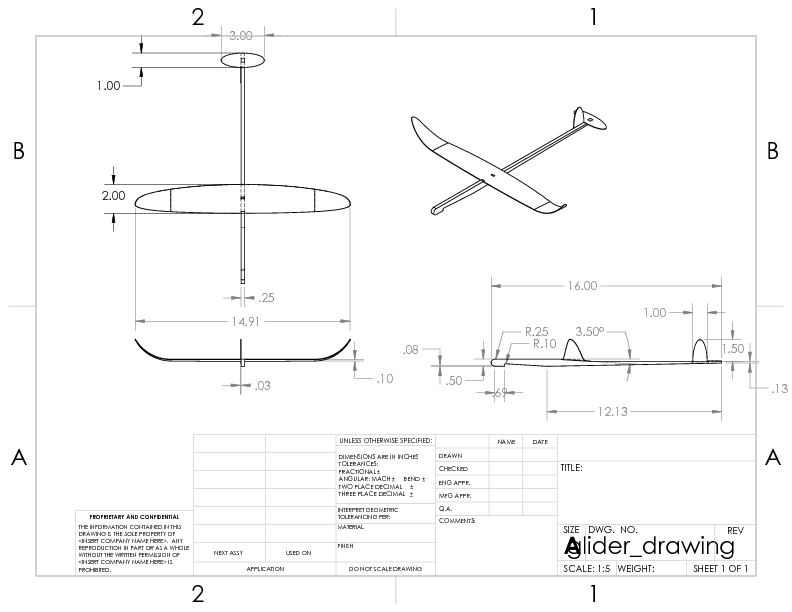
\includegraphics[width = \linewidth]{glider_drawing.png}

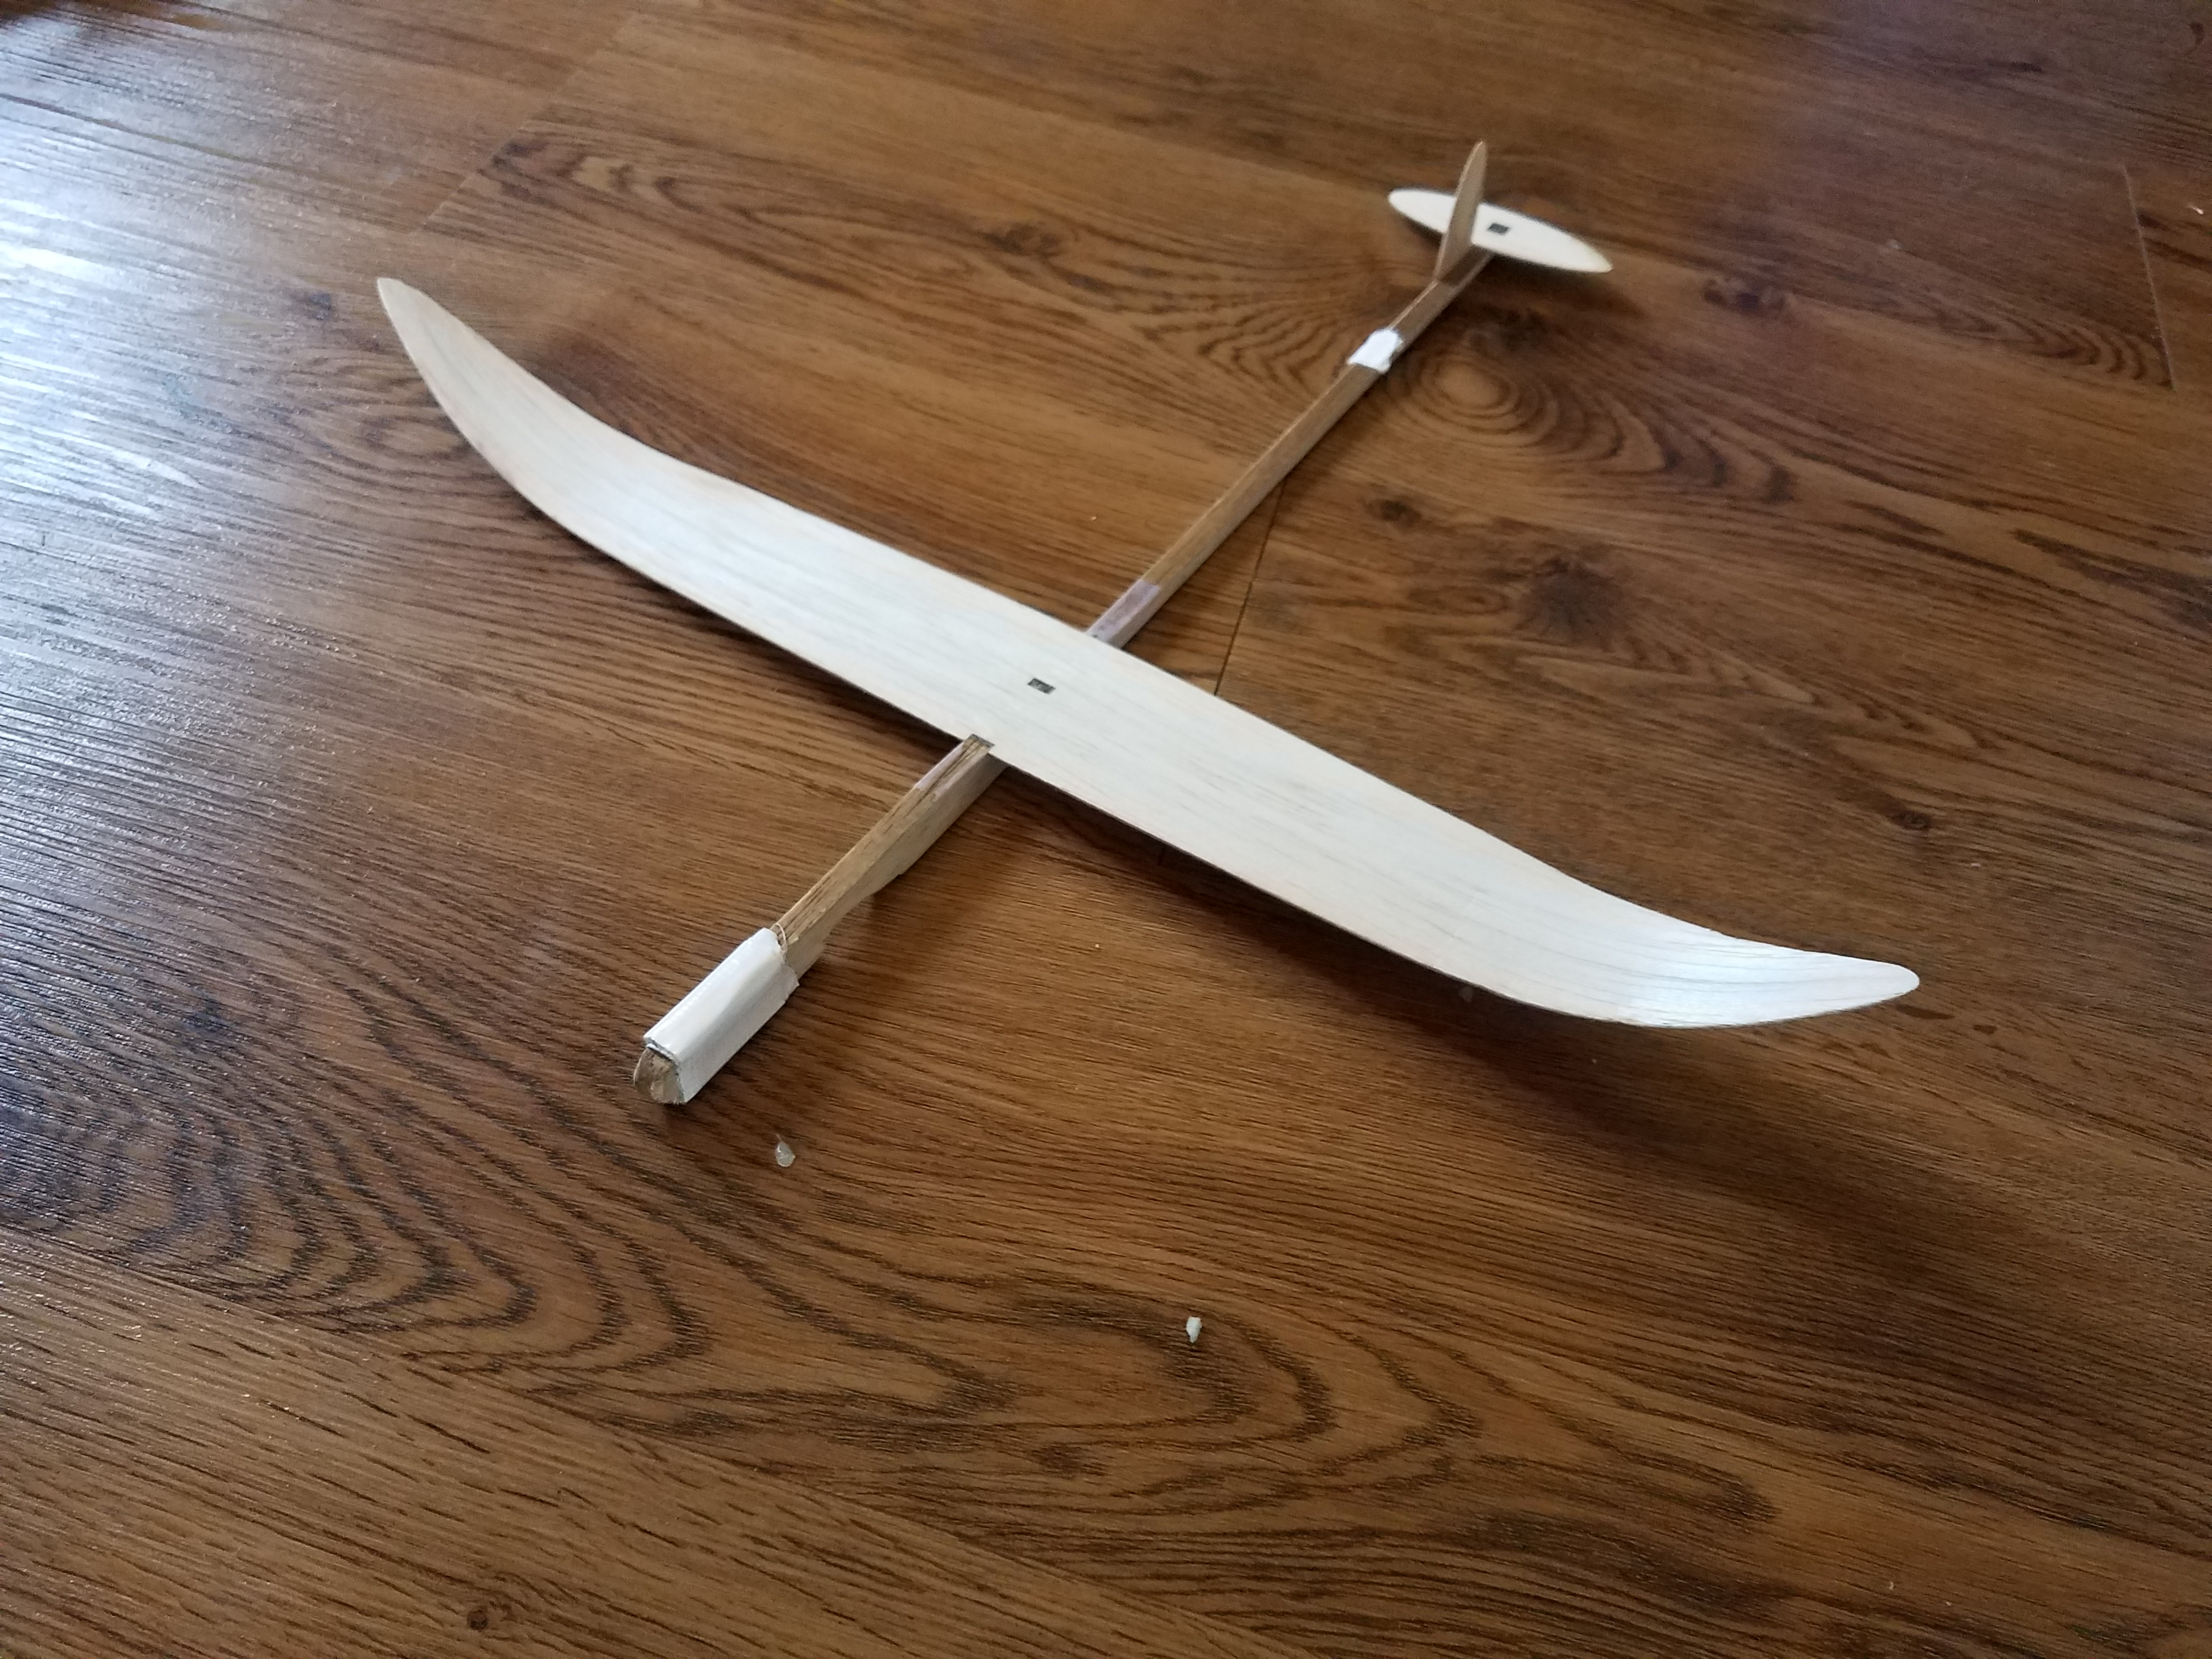
\includegraphics[width = \textwidth]{glider.jpg}

\section{Analysis of Lift and Drag}

Note: Unconventionally, this section comes before "Weight and Balance". This is because, unlike powered aircraft, for this glider the results
of lift and drag analysis were essential to the
selection of the aircraft weight. Because our wing span and chord were already determined based on sizing constraints defined in the competition
rules, we were able to discern that Re would be very small. In order to compute lift and drag, XFOIL was run using the NACA 0002 airfoil, whose
thickness-to-chord ratio is similar to that of our 1/32" thick by 2" max chord wing. Rudimentary analysis in XFOIL demonstrated that for
velocity less than 10m/s, changes in velocity lead to changes in Re which had a significant impact on lift and drag. Thus it was determined
that Re, and hence the speed, were important considerations in our design.

Since we are required to launch from a specified height, and the
objective is to maximize the horizontal distance traveled, it was assumed that the optimal trajectory is to launch the glider at its equilibrium
glide conditions, i.e. such that the glider will fly at a constant velocity until it strikes the ground (this assumption is not necessarily
accurate, but at the time of the design it was not known who would launch the glider and how much energy they would impart to it, so we opted
to simply optimize the glider in equilibrium and hope it was closed to optimized for the actual mission). Basic physics shows that

\[m = \frac{L}{D} = \frac{C_L}{{C_D}_0 + {C_D}_i}\]
(I am not sure if this is common knowledge, but if it is difficult to see, draw a free body diagram, and notice that the vector representing
the weight force forms the hypotenuse of a right triangle whose other sides are L and D.)

So the goal is to maximize L/D. Assuming that ${C_D}_0$ is fixed, $C_L$ varies linearly with $\alpha$, and ${C_D}_i = \frac{C_L^2}{\pi AR e}$,
some calculus was done derive an optimum value of $\alpha$ to maximize L/D. However, after it turned out that the optimum predicted by this model
would cause the wing to stall, which invalidates the assumptions. So, instead, an approximate optimum was found by generating drag polars in XFOIL
for each Re and selecting the value of $\alpha$ which maximizes $frac{C_L}{{C_D}_0}$. At such an $\alpha$, it was found that ${C_D}_i$ is small,
indicating that this optimum is close to the actual optimum. Thus we had a method for designing the angle of attack for any given Re.

Exploration in XFOIL also showed that for speeds less than 10m/s, the ratio $\frac{C_L}{{C_D}_0}$, increases as Re increases. So, we may achieve
better performance by increasing the speed. However, there is a limit to how fast we may design our glider to go. While it may be optimal to
launch our glider at the speed of a bullet, this would not be achievable using a rubber band launcher. In order to select a speed, a set of
Re values were selected. For each Re, XFOIL was run and the optimum $\alpha$ was computed. Then, $C_L, {C_D}_0$, and ${C_D}_i$ were computed
and used to find m. Also, based on our chord, for each Re the speed at which the aircraft would have to fly in order to attain that Re was
computed. Re = 11500, giving V = 4.3m/s was selected as the highest (and therefore best) speed which was feasible with a rubber band launcher. The
optimim $\alpha$ was discovered to be 3.5\degree.

\section{Weight and Balance}

Again, basic physics shows that when the glider is in equilibrium,

\[W = \sqrt{L^2 + D^2}
= \frac{1}{2}\rho V^2 \sqrt{C_L^2 + ({C_D}_0 + {C_D}_i)^2}\]

So, from our selected Re, it is possible to determine the targe weight which will achieve the desired equilibrium glide speed. This target weight
turns out to be 8.3g. It was determined that the CG should be at the quarter chord of the wing. Based on thin airfoil theory, the main wing should
generate lift at one quarter of the chord length from the leading edge (from

\verb|http://www2.esm.vt.edu/~dtmook/AOE5104_ONLINE/Class|

\verb|%20Notes/19_Class_ThinAirfoilTheory.pdf|. This gives "$cp_x$" in terms of some fourier coefficients, but those coefficients should be zero for a symmetric airfoil). So, if
we place the CG there, all of the lift will be generated by the main wing, with the tail contributing only to bring the aircraft back to trim if it
is disturbed by a gust, or imperfect launch. This is what we want, as the tail will have a lower aspect ratio, so it will generate more drag for
a given amount of lift.

So, it was
assumed that some ballast would need to be added to strategic locations in order to influence the CG. So, the balsa parts were designed as light
as possible, so that ballast could be added to bring the weight up to the proper value. Due to the importance of ballast, there was no "calculated"
center of mass. It was decided that the center of mass would occupy a point 1/4 of the chord length from the leading edge of the wing. Ballast was
added to the nose until the plane, when supported by two points in line with the target CG location, it would balance. This is the extent of CG
calculations and measurements.

The breakdown of component weight is as follows:

\begin{tabular}{|l | c|}
\hline
Component & mass (g) \\ \hline
Wing & 2.05\\
Fuselage & 3.14\\
Horizontal Stabilizer & 0.19\\
Vertical Stabilizer & 0.11\\
Ballast and Adhesives 2.22\\ \hline
Total & 7.7\\ \hline
\end{tabular}

\section{Trim and Stability}

The following were taken as common knowledge:
\begin{itemize}
\item The CG should be in front of the aerodynamic center
\item The glider should include a vertical stabilizer in the rear for directional stability
\item The glider should either have its CG below the main wing or di/polyhedral for roll stability
\end{itemize}

By placing the CG at the quarter chord of the wing and including a horizontal stabilizer, the CG was made to be in front of the aerodynamic center.
It was assumed that the tail should be made as small as possible to minimize drag. So, the horizontal stabilizer was made to be 3 inches span by 1
inch chord. It was positioned to give a static margin of 0.45. Based off of

\verb|ocw.mit.edu/courses/aeronautics-and-astronautics/16-01-unified-|

\verb|engineering-i-ii-iii-iv-fall-2005-spring-2006/systems-labs-06/spl8.pdf|
this seems to be an acceptably high number. The wingtips were curved upward to provide roll stability.

In order to trim the aircraft, ballast was added to the nose until the CG was in the target location. The aircraft was tested to verify that it
flew as expected. On one of the prototypes, the CG was experimentally adjusted, but as expected no improvement could be achieved.

\section{Design Process}
For the design, the designers chose the maximum length for the fuselage of the glider because a longer fuselage allows for an easier alteration of the center of mass as needed and is generally more stable than a shorter a glider with a shorter fuselage. To increase the stability of the glider, the designers chose to curve the tip of the wings up which also in-turn reduces induced drag by eliminating/ reducing the occurrences of a vortex at the tip of the wing. They also chose an elliptical wing design because an elliptical wind lift distribution allows for the lowest induced drag. There were not that many alterations made to the original design besides the experimentation of the placement of the center of mass. 

In order to determine the target weight, an Excel spreadsheet was used. The wing length and overall length was set to be the maximum allowed by
the rules. The chord was set to be 2" based off of intuition that it was as small as we could reasonably go (and as small as possible in order to
maximize AR). Then, for a series of Reynolds numbers, the speed necessary to achieve that number was computed, and $C_L$ and ${C_D}_0$ obtained from
XFOIL. Then, using equations outlined above, the weight needed to achieve that speed was computed. The ratio L/D was used to stand in for the score
(since it defines the glide slope and therefore the distance traveled). It was observed that higher speeds yielded higher scores, but would be
more difficult to achieve with a throw. 4.3g was selected as the weight in order to balance these two factors. The spreadsheet is included in the
appendix.

1/32" Balsa was used for the wing, because increasing the thickness would increase the drag. The fuselage was made as narrow as possible in order to
minimize drag. The tail was made as small as possible while still achieving static stability. It was hoped that maintaining non-excessive amounts
of longitudinal and directional static stability would provide phugoid and spiral stability.

\section{Testing and Evaluation}
From the four-trial conducted, the longest range for this given glider was roughly 85 feet. The designers conducted several pretests prior to the final launch day with the final glider design. From the several pretests conducted, the longest range was roughly 50 feet. The designers launched the glider from a height of 6 feet above the ground during the pretests and the glider was thrown by hand for the pretest trials. The final launch, however, took place from a height of a one story high platform, around 3 meters in height, and the designers employed rubber bands to launch the craft, hence the discrepancy between the pretest and final run. The pretests were also conducted outdoors with wind in effect while the final run was conducted indoors. 

A spreadsheet was used to predict the glider's performance. When using the profile drag predicted by XFOIL, the predicted performance was
greater than the actual by about 20\%. However, when the profile drag is increased, the spreasheet can be made to predict the glider's
performance to within about 5' (less than 10\% error). This indicates that the actual ${C_D}_0$ was about 0.055, rather than the 0.043 which XFOIL
predicted. The improved spreasheet is included in the appendix.

\section{Conclusion and Recommendations for Further Improvement}
The designed tried to maximize the range of the glider is able to travel by reducing drag and by design a stable glider. An elliptical wing design was selected for its efficiency when it comes to reduced induced drag. To further reduce induced drag caused by vortexes, the designers decided to curve the ends of the wing, which would reduce/ eliminate induced drag. The dimensions for the gliders were chosen to optimize stability while giving the designers greater control over the placement of the center of mass. The calculations prior to testing were done in an excel spreadsheets, which had outputs the like of range of the glider was able to travel. The designers’ calculation predicted that the glider would be able to travel a distance of 88 feet; during the final testing, however, the glider traveled a maximum distance of. 85 feet from the four trials. The discrepancy between the actual value and predicted value might be due a little difference in the force applied by the person launching the glider- using a rubber band, the height from which the glider was released
from, and other human errors might have influenced the actual result. If there was another iteration to this projects, the designers would add a "T-tail". This is based on the observation that T-tails tended to perform very well at the fly off. Perhaps this is because it raises the GC from the center of the fuselage, further increasing the stability of the glider. Or, it could be that it moves the tail out of the turbulent flow from the wing, reducing drag.

\section{Appendix}
\subsection{Trajectory Calculation}
\begin{minipage}{0.5\linewidth}
	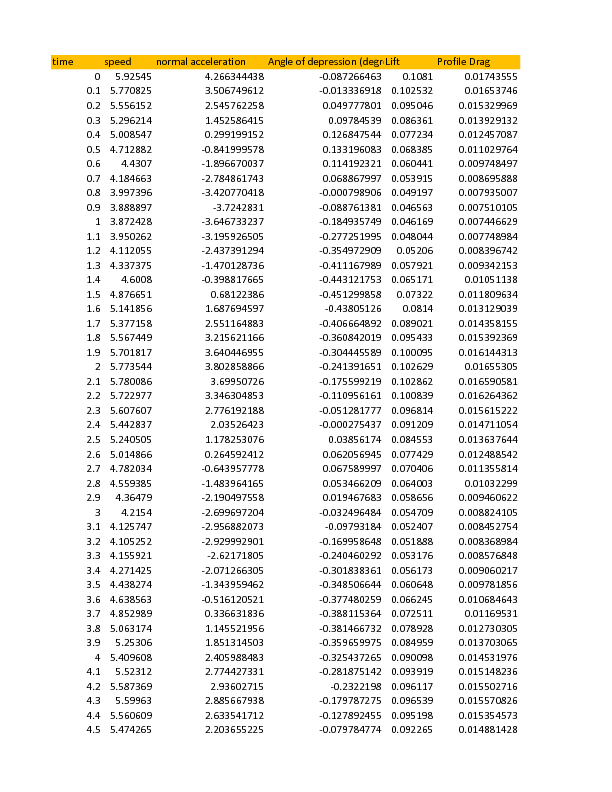
\includegraphics[width = \textwidth]{glider_trajectory-0.png}
\end{minipage}
\begin{minipage}{0.5\linewidth}
	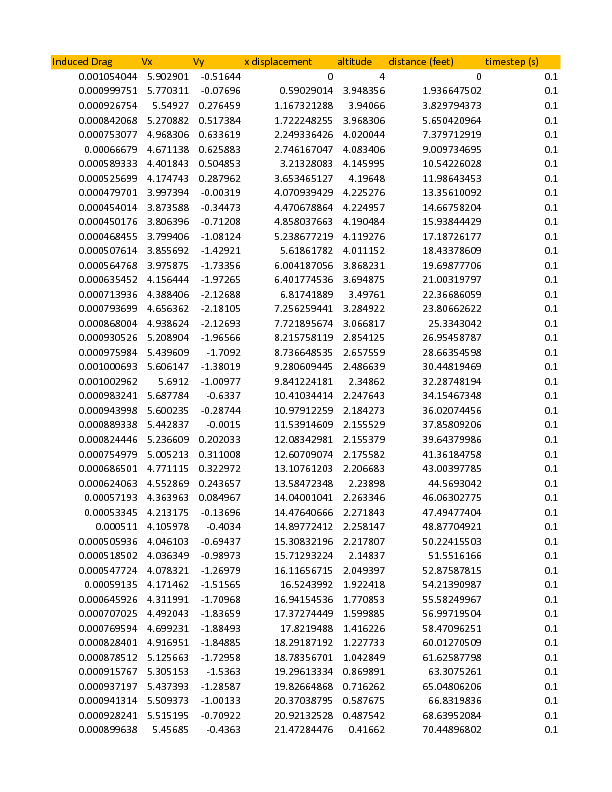
\includegraphics[width = \textwidth]{glider_trajectory-5.png}
\end{minipage}
\begin{minipage}{0.5\linewidth}
	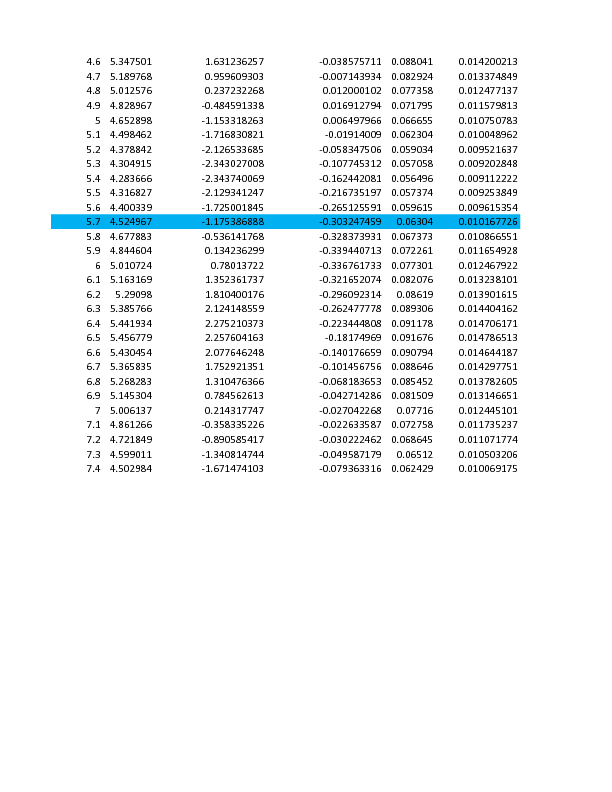
\includegraphics[width = \textwidth]{glider_trajectory-1.png}
\end{minipage}
\begin{minipage}{0.5\linewidth}
	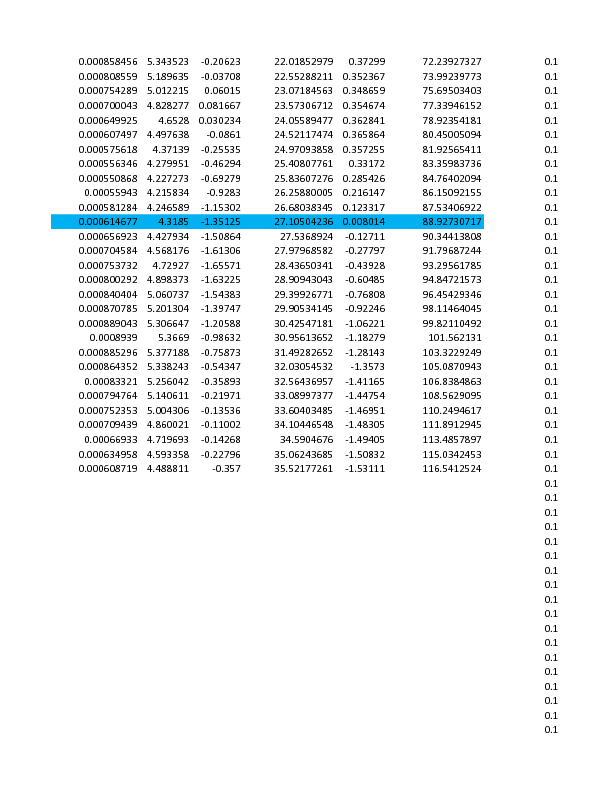
\includegraphics[width = \textwidth]{glider_trajectory-6.png}
\end{minipage}
\subsection{Weight optimization}
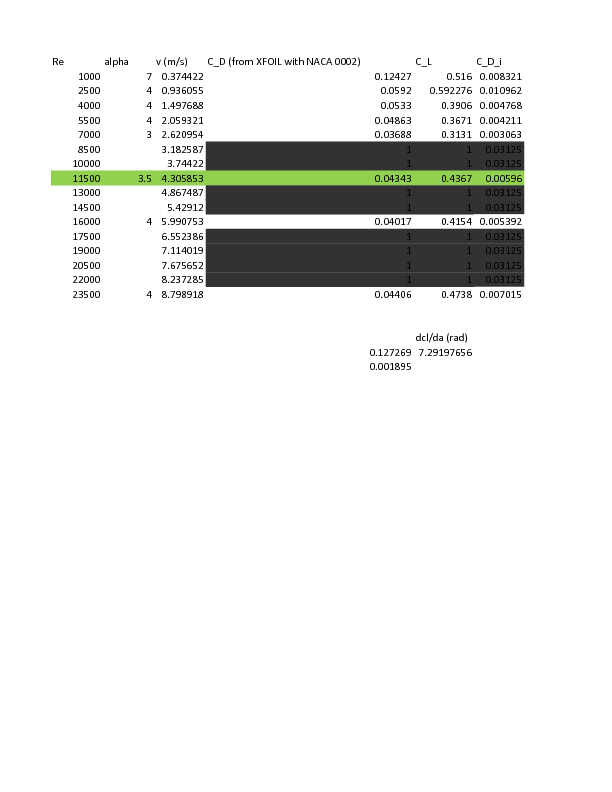
\includegraphics[width = \textwidth]{glider_weight_calculation-0.png}
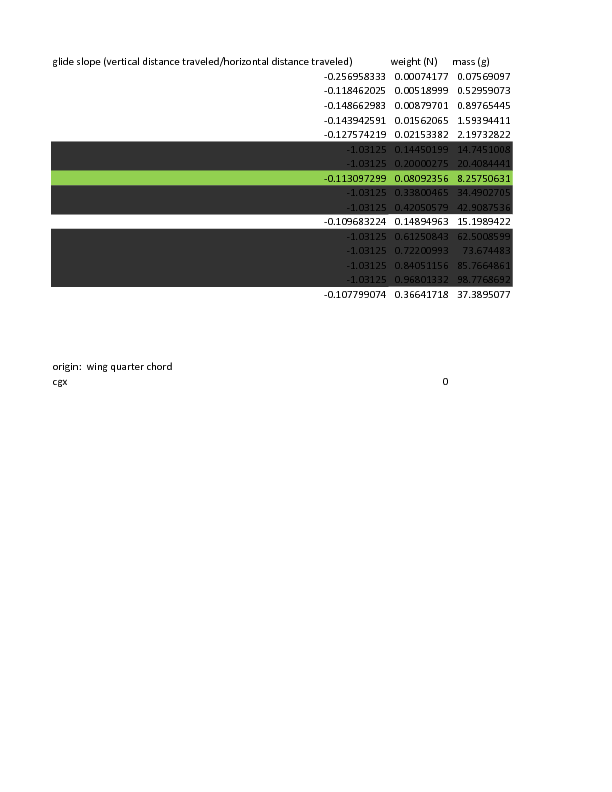
\includegraphics[width = \textwidth]{glider_weight_calculation-1.png}
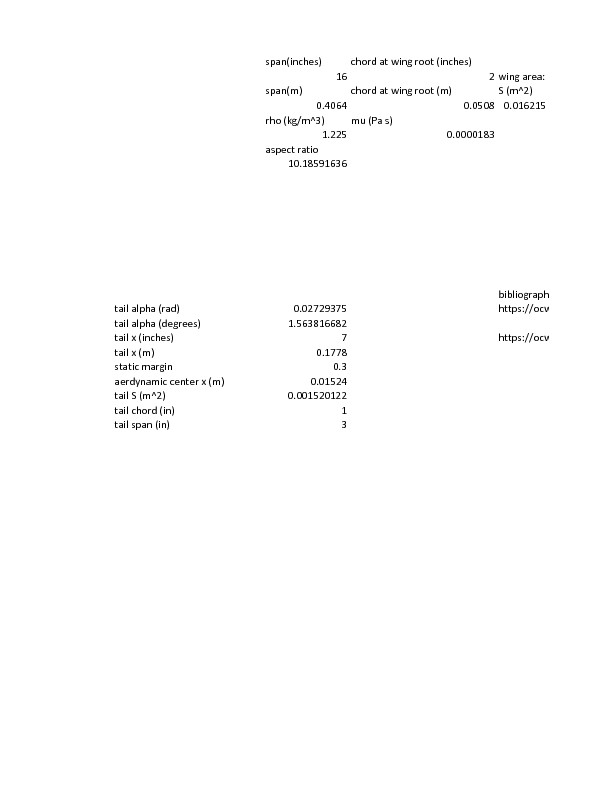
\includegraphics[width = \textwidth]{glider_weight_calculation-2.png}


\section{References}

\begin{itemize}
\item \verb|ocw.mit.edu/courses/aeronautics-and-astronautics/16-01-unified-|

\verb|engineering-i-ii-iii-iv-fall-2005-spring-2006/systems-labs-06/spl8.pdf|





\item \verb|http://www2.esm.vt.edu/~dtmook/AOE5104_ONLINE/Class|

\verb|%20Notes/19_Class_ThinAirfoilTheory.pdf|

\end{itemize}
\end{document}
